\section{Выбор решателя задач целочисленного линейного программирования}
\label{sec:4_solvers} \index{4_solvers}


\subsection{Обзор решателей}\label{sec:solvers_overview}


Существует ряд программных средств решения задачи ЦЛП (далее –
«решатели»). Выбор решателя для использования в данной работе основан на
критериях доступности, поддержки основных программных платформ и наличия входного языка «lp» для описания задач ЦЛП.
Рассмотрение решателей ЦЛП по этим критериям приведено в таблице \ref{overview}.

\begin{table}[h!]
    \caption{\label{overview}Обзор решателей ЦЛП}
    \begin{tabular}{|> {\centering\arraybackslash} p{3.8cm}|> {\centering\arraybackslash} p{4.5cm}|c|p{2cm}|} \hline 
        \centering\arraybackslash \textbf{Решатель} & \centering\arraybackslash\textbf{Доступность} & \textbf{Платформа} & 
        \textbf{Наличие входного языка lp} \\ \hline 
        CBC COIN-OR \cite{COIN} & свободный доступ, Eclipse Public License & Linux, Windows, MacOS & \centering\arraybackslash + \\ \hline 
        GLPK (GNU Linear Programming Kit) \cite{GLPK} & свободный доступ, GNU General Public License (GPL) & Linux, Windows, MacOS & \centering\arraybackslash + \\ \hline 
        SCIP \cite{SCIP} & свободный доступ, Apache License & Linux, Windows, MacOS & \centering\arraybackslash + \\ \hline 
        HiGHS \cite{HiGHS} & свободный доступ, MIT License & Linux, Windows, MacOS & \centering\arraybackslash + \\ \hline 
        GAMS \cite{GAMS} & есть академическая
лицензия, но она не
доступна в РФ & Linux, Windows, MacOS & \centering\arraybackslash + \\ \hline
        GUROBI \cite{GUROBI}  & есть академическая
лицензия, но она не
доступна в РФ & Linux, Windows, MacOS & \centering\arraybackslash + \\ \hline 
    \end{tabular}
    \label{tab:my_label}
\end{table}

Из свободно доступных решателей для сравнения производительности были выбраны GLPK, SCIP, CBC COIN-OR, поскольку они удовлетворяют всем критериям. Решатель HiGHS был найден и добавлен в обзор после выполнения основного объема экспериментов, поэтому в сравнении производительности не участвовал.


\subsection{Формирование входных данных решателя}\label{sec:input_generation}

Соответствующие входному графу $G$ линейные ограничения необходимо
транслировать во входной язык решателя, в данном случае -- язык «lp». При трансляции необходимо
распределить переменные и линейные ограничения по секциям входного
файла решателя:

\begin{itemize}
    \item переменные -- по секциям Integer и Binary (см. таблицу \ref{tab:variable_distribution})

    \item ограничения -- по секциям Subject to и Bounds (см. таблицу \ref{tab:restrictions_distribution})
\end{itemize}

Целевая функция, равная переменной F, находится в секции Minimize.

\begin{table}[h]
    \caption{Распределение переменных задачи по секциям}
    \centering
    \begin{tabular}{|c|>{\centering\arraybackslash}p{6.5cm}|>{\centering\arraybackslash}p{6.5cm}|}
    \hline
    \textbf{Секция} & \textbf{Переменные формальной постановки} & \textbf{Переменные на входном языке решателя} \\ 
    \hline
    Integer & $F, s_j$ & F, s\_j \\ 
    \hline
    Binary & $m_{ij}, w_{ij}, l_{ij}$ & m\_i\_j, w\_i\_j, l\_i\_j \\ 
    \hline
    \end{tabular}
    \label{tab:variable_distribution}
\end{table}


\begin{table}[h]
    \caption{Распределение ограничений задачи по секциям}
    \centering
    \begin{tabular}{|l|l|}
    \hline
    \textbf{Секция} & \textbf{Линейные ограничения формальной постановки} \\ 
    \hline
    Subject to & (1), (2), (4), (5), (7), (10), (11), (12) \\ 
    \hline
    Bounds & (3), (6), (8), (9) \\ 
    \hline
    \end{tabular}
    \label{tab:restrictions_distribution}
\end{table}


\begin{figure}[h!]
    \centering
    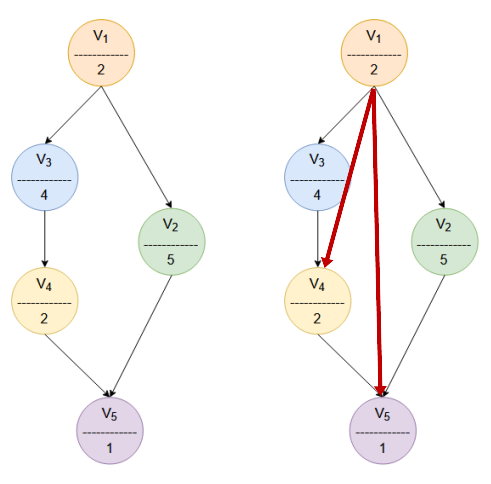
\includegraphics[width=0.7\linewidth]{pictures/transitive_edges.png}
    \caption{Добавление транзитивных ребер}
    \label{fig:transitive_edges}
\end{figure}

Предварительные прогоны решателей показали, что время получения результата может быть сокращено путем добавления транзитивных ограничений частичного порядка на множестве вершин графа. А именно, если $(p_i, p_j) \in E$ и $(p_j, p_k) \in E$, добавляется ограничение вида (3), как если бы $(p_i, p_k) \in E$. Ограничения такого вида не изменяют множество допустимых решений, поскольку не добавляют новых ограничений частичного порядка. 

Предварительные прогоны проводились на процессоре, описанном в подразделе \ref{sec:results}.

\begin{figure}[h!]
    \centering
    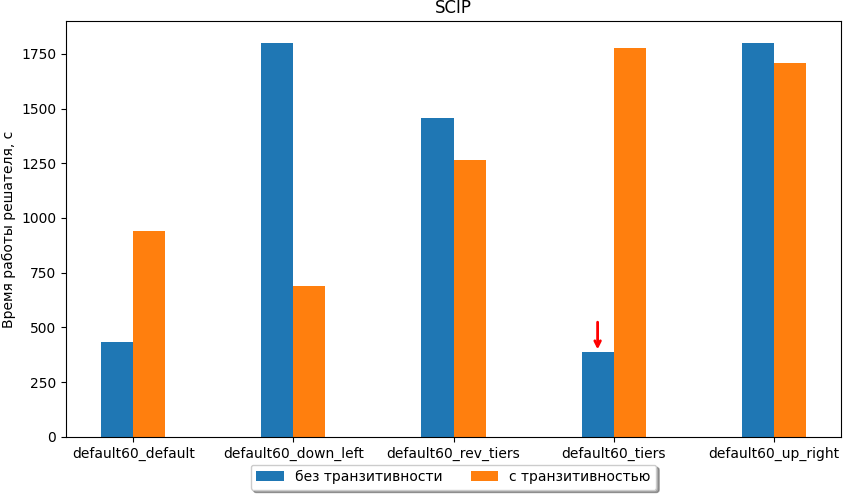
\includegraphics[scale=0.53]{pictures/default60.png}
    \caption{Преимущество сведения без транзитивности.}
    \label{fig:default60}
\end{figure}

\begin{figure}[h!]
    \centering
    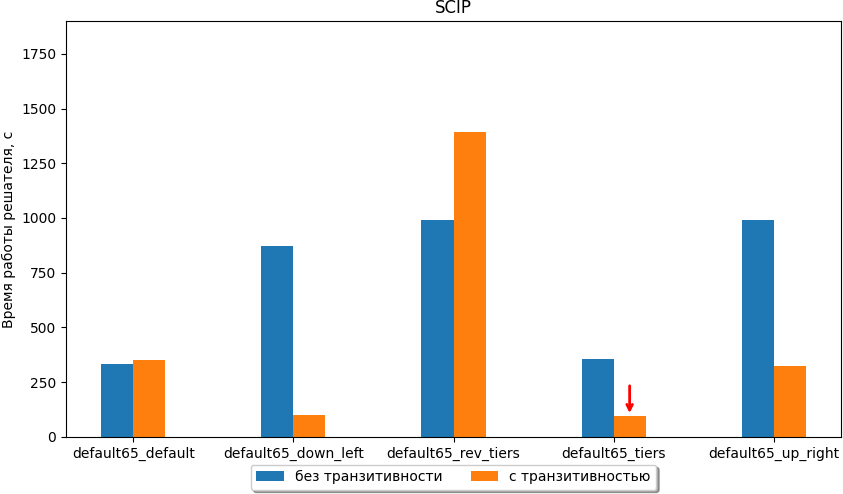
\includegraphics[scale=0.53]{pictures/default65.png}
    \caption{Преимущество сведения с транзитивностью.}
    \label{fig:default65}
\end{figure}

На рис. \ref{fig:transitive_edges} показан исходный граф (слева) и граф с добавленными ребрами, соответствующими транзитивным ограничениям (далее для краткости -- граф с транзитивностью).

На диаграммах (рис. \ref{fig:default60}, \ref{fig:default65}) сравнивается время нахождения решателем SCIP решения с одними и теми же входными данными задачи, на графах с наличием и отсутствием транзитивных ребер и различными упорядочениями вершин и ребер. Красной стрелкой показан результат с наименьшим временем выполнения. На рис. \ref{fig:default60} показан случай, в котором решение находится быстрее при отсутствии транзитивности, а на рис. \ref{fig:default65} случай, в котором решение находится быстрее при наличии транзитивности. 

Предварительные прогоны также показали, что время получения результата зависит от порядка перечисления вершин и ребер графа, а соответственно –- от порядка следования переменных и ограничений в секциях входного файла
решателя. В терминах файла с описанием графа работ, порядок перечисления
вершин –- это порядок строк в файле; порядок вершин в строке –- это порядок
перечисления в строке потомков вершины, т.е. исходящих ребер. Ниже приведен
пример файла с описанием графа, в нем поле node соответствует вершине
графа, поле size –- занимаемому ресурсу, поле children –- потомкам данной
вершины:
\begin{table}[h]
    \centering
    \begin{tabular}{ccc}
        node & size & children \\
        \hline
        1 & 2 & 2 3 \\
        2 & 5 & 3 \\
        3 & 4 &   \\
    \end{tabular}
    \label{tab:sample_data}
\end{table}

В данной работе использовались следующие варианты упорядочения: 

\begin{enumerate}
    \item \textit{default}: проход по строкам (имеются в виду строки входного файла с описанием графа) сверху вниз, по вершинам в строке слева
направо;

    \item \textit{down\_left}: проход по строкам сверху вниз, по вершинам в строке справа
налево;

    \item \textit{up\_right}: проход по строкам снизу вверх, по вершинам в строке слева
направо;

    \item \textit{tiers}: строки упорядочены по возрастанию номера яруса, к которому
относится вершина, вершины одного яруса упорядочены по
возрастанию номеров в первоначальном файле; в каждой строке вершины-потомки упорядочены
по той же схеме;

    \item \textit{reverse\_tiers}: схема, обратная к tiers, причем ярусы отсчитываются
начиная с выходных вершин графа.
\end{enumerate}

На рис. \ref{fig:sorts} и рис. \ref{fig:sorts_tr} сравнивается время работы решателя SCIP в зависимости от упорядочения входных данных при отсутствии и наличии транзитивности соответственно. Каждая группа из пяти столбцов соответствует одному графу с разными упорядочениями. Прогоны решателя для каждого из этих рисунков прерывались, если за 1 час не был получен результат. Тем самым, длительность прогона в 3600 секунд соответствует отсутствию результата. Красной стрелкой отмечено упорядочение с наименьшим временем нахождения решения.

На рис. \ref{fig:sorts} и рис. \ref{fig:sorts_tr} видно, что время работы решателя очень существенно (в разы, в десятки раз) различается в зависимости от упорядочения входных данных. 

\begin{figure}[h!]
    \centering
    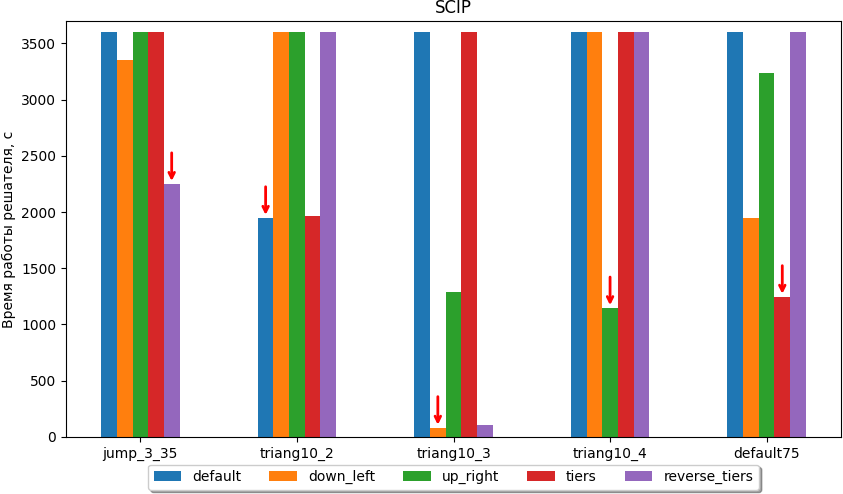
\includegraphics[scale=0.49]{pictures/sorts.png}
    \caption{Зависимость времени работы решателя от упорядочений для графов без транзитивности.}
    \label{fig:sorts}
\end{figure}

\begin{figure}[h!]
    \centering
    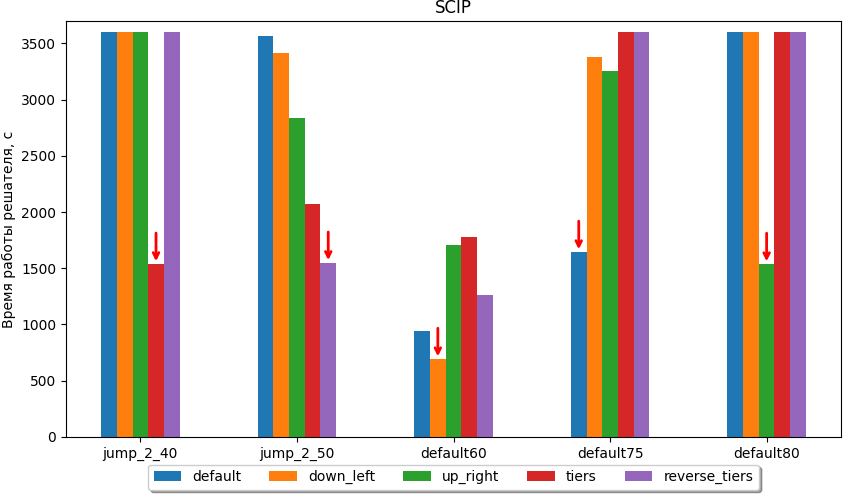
\includegraphics[scale=0.49]{pictures/sorts_tr.png}
    \caption{Зависимость времени работы решателя от упорядочений для графов с транзитивностью.}
    \label{fig:sorts_tr}
\end{figure}


\newpage
\subsection{Сравнение производительности решателей}\label{sec:solvers_benchmark}

Были проведены предварительные эксперименты для решателей SCIP 9.2.1, GLPK 5.0, CBC COIN-OR 2.10.12 на всех классах графов с лимитом времени 1800 секунд. Подробное описание классов графов можно прочитать в подразделе \ref{sec:data_classes}.

Предварительные эксперименты проводились на компьютере со следующими характеристиками:
\begin{itemize}
    \item ЦП: AMD Ryzen 3 5300U, тактовая частота 2.6 ГГц
    \item Количество ядер: 4
    \item Oбъем ОЗУ: 8 Гб
    \item OС: Ubuntu 20.04 LTS
\end{itemize}

Результаты экспериментов представлены на рис. \ref{fig:solvers_default} -- \ref{fig:solvers_dag}. Графы на каждой диаграмме упорядочены в порядке возрастания количества вершин (соответствуют числам в конце названия графа). Цвету столбца соответствует наличие/отсутствие транзитивных ограничений на том варианте входных данных, где расчет у данного решателя завершился раньше всего, а цвету границы столбца –- упорядочение вершин и ребер. Над каждым столбцом на диаграмме находится буква, соответствующая первой букве названия решателя: G –- GLPK, C –- CBC, S –- SCIP. 

\begin{figure} [h!]
    \centering
    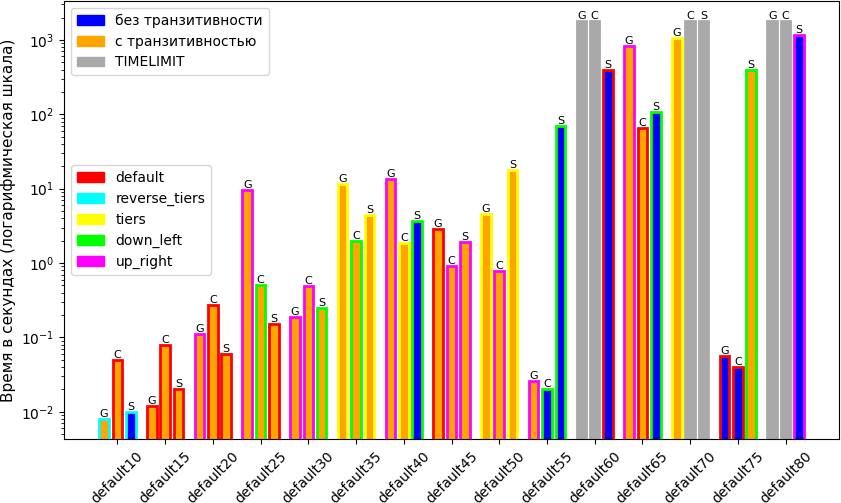
\includegraphics[width=0.85\linewidth]{pictures/solvers_default.png}
    \caption{Время выполнения решателей на слоистых графах с числом «пропускаемых слоев» 0.}
    \label{fig:solvers_default}
\end{figure}

\begin{figure} [h!]
    \centering
    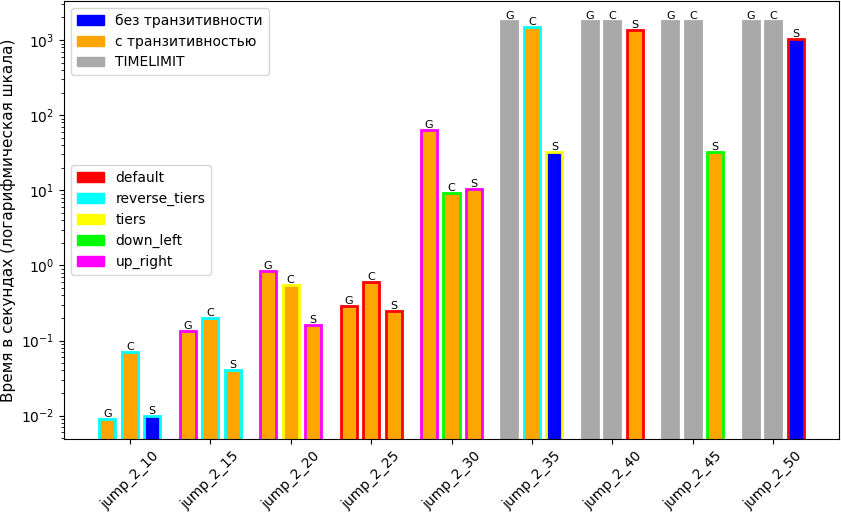
\includegraphics[width=0.85\linewidth]{pictures/solvers_jump2.png}
    \caption{Время выполнения решателей на слоистых графах с числом «пропускаемых слоев» 1.}
    \label{fig:solvers_jump2}
\end{figure}

\begin{figure} [h!]
    \centering
    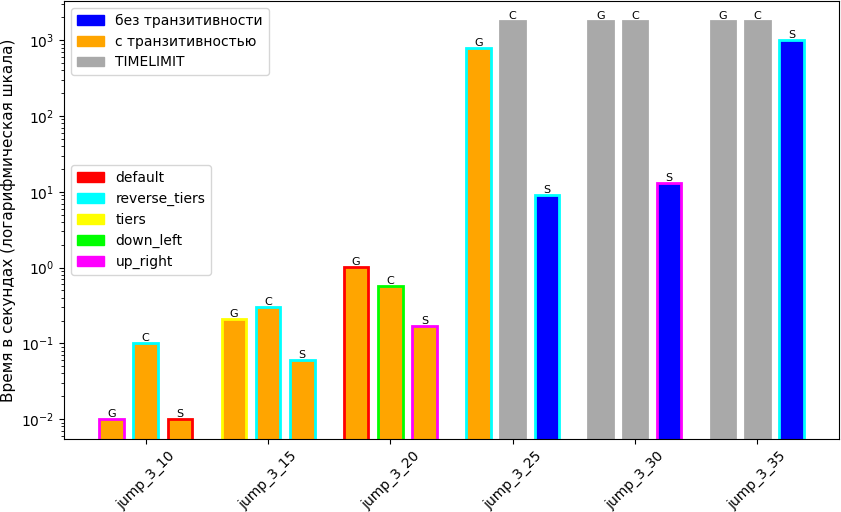
\includegraphics[width=0.85\linewidth]{pictures/solvers_jump3.png}
    \caption{Время выполнения решателей на слоистых графах с числом «пропускаемых слоев» 2.}
    \label{fig:solvers_jump3}
\end{figure}

\begin{figure} [h!]
    \centering
    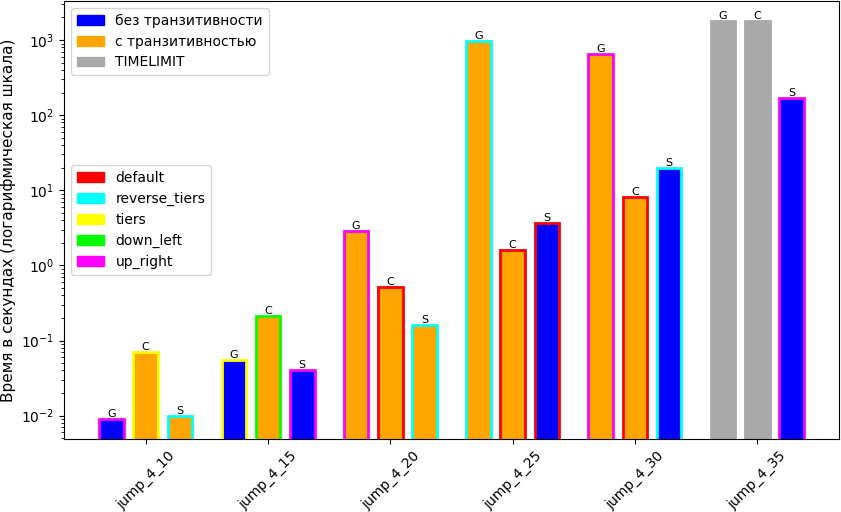
\includegraphics[width=0.85\linewidth]{pictures/solvers_jump4.png}
    \caption{Время выполнения решателей на слоистых графах с числом «пропускаемых слоев» 3.}
    \label{fig:solvers_jump4}
\end{figure}

Диаграммы на рис. \ref{fig:solvers_default} -- \ref{fig:solvers_jump4} соответствуют слоистым графам. Графы, название которых начинается на jump\_2, jump\_3, jump\_4, имеют количество слоев, пропускаемых ребрами, соответственно 1, 2 и 3. Для графов, название которых начинается на default, пропускаемые слои отсутствуют. 

По диаграмме рис. \ref{fig:solvers_default} однозначный выбор решателя для слоистых графов сделать сложно. Так, например, SCIP на default60 и default80 единственный не достигает лимита времени, но на default55 и default75 превышает лучшее время выполнения в сотни раз. В то же время, по диаграммам рис. \ref{fig:solvers_jump2} -- \ref{fig:solvers_jump4} можно сделать однозначный выбор в пользу SCIP, так как он чаще завершается раньше остальных и реже превышает лимит времени.

\begin{figure} [h!]
    \centering
    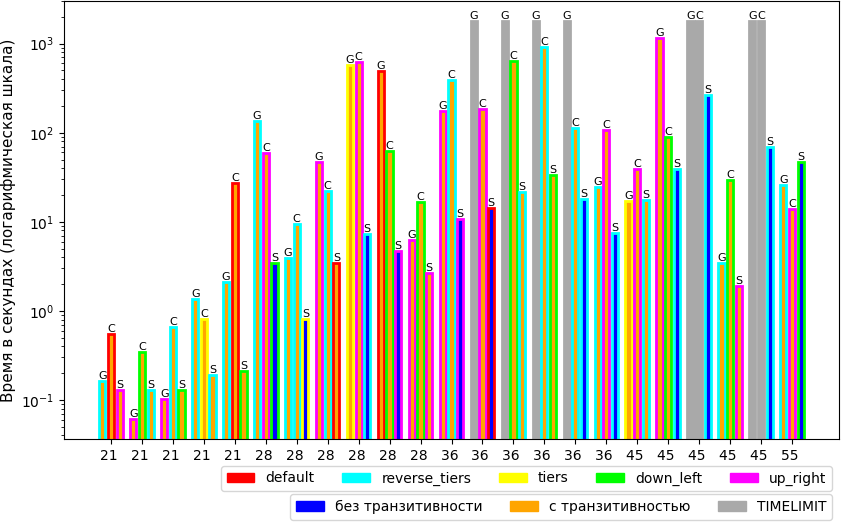
\includegraphics[width=0.918\linewidth]{pictures/solvers_triang.png}
    \caption{Время выполнения решателей на треугольных графах.}
    \label{fig:solvers_triang}
\end{figure}

На диаграмме рис. \ref{fig:solvers_triang} для треугольных графов видно, что SCIP в большинстве случаев завершается быстрее (зачастую в $\approx10$ раз) других решателей и, в отличие от них, ни разу не достигает лимита времени выполнения. 

\begin{figure} [h!]
    \centering
    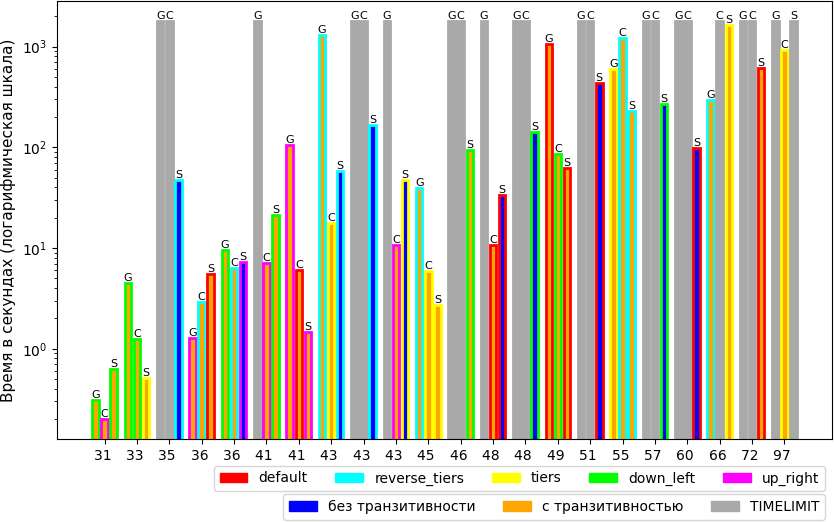
\includegraphics[width=0.9\linewidth]{pictures/solvers_dag.png}
    \caption{Время выполнения решателей на случайных графах.}
    \label{fig:solvers_dag}
\end{figure}

На случайных графах (см. рис. \ref{fig:solvers_dag}) ситуация аналогична ситуации с треугольными графами.


\subsection{Выводы}
По совокупности проведенных экспериментов решатель SCIP оказался лучшим по скорости решения задач, поэтому дальнейшие эксперименты проводились на нем. При этом целесообразно запускать решатель с разными упорядочениями и как наличием, так и отсутствием добавленных транзитивных ребер в графе.